\fancypagestyle{headings}{
    \fancyhf{}
    \fancyfoot[C]{\songti\xiaowu 第 \thepage 页}
    \fancyhead[L]{\songti\xiaowu 上海工程技术大学硕士学位论文}
    \fancyhead[R]{\songti\xiaowu 第\zhnum{chapter} 章 \quad 课题研究}
}
\pagestyle{headings}
\chapter{举个例子:粒子群算法(matlab实现)}
\section{基本原理}
\subsection{算法概括}
粒子群算法(PSO),在PSO中,每个优化问题的潜在解都是搜索空间的一只鸟,被称为粒子,所有的粒子都有一个由适应度函数决定的适值,每个粒子还有一个速度决定它们“”飞行“”的方向和距离,然后粒子们就追随当前的最优粒子在解空间中搜索,整个过程大致为,PSO初始化为一群随机粒子(随机解),然后通过迭代找到最优解。在每一次迭代的过程中,粒子通过跟踪两个极值来更新自己:第一个就是粒子本身所找到的最优解,这个解称为个体极值;另一个极值是整个种群目前找到的最优解,这个解是全局极值。
\subsection{式子说明}
假设在一个$D$维度的目标搜索空间中,有$N$个例子组成一个群落,其中第$i$个例子表示为一个$D$维度向量
\begin{eqnarray}
    X_{i}&=&\left(x_{i1},x_{i2},\cdots,x_{iD}\right),i=1,2,\cdots,N
\end{eqnarray}

第$i$个例子的“飞行”速度也是一个$D$维度向量,记作以下的形式:
\begin{eqnarray}
    V_{i}&=&\left(v_{i1},v_{i2},\cdots,v_{iD}\right),i=1,2,\cdots,N
\end{eqnarray}

第$i$个例子迄今为止搜索到的最优位置称为个体极值,记作
\begin{eqnarray}
    P_{\text{best}}&=&\left(P_{i1},P_{i2},\cdots,P_{iD}\right),i=1,2,\cdots,N
\end{eqnarray}

整个粒子群迄今为止搜索到的最优位置为全局极值,记作
\begin{eqnarray}
    g_{\text{best}}&=&\left(P_{g1},P_{g2},\cdots,P_{gD}\right)
\end{eqnarray}

解释:如果是求一个有三个变量的杉树极值为题,则$D$维值得就是三维,$X_{i}$指的就是某一点坐标,$V_{i}$也是三维的,用于改变当前坐标,$P_{\text{best}}$也是一个坐标,是当前粒子最优位置坐标,$g_{\text{best}}$也是一个坐标,是当前整个粒子群最优位置坐标。

在找到这两个最优值时,粒子根据如下公式来更新自己的速度和位置:
\begin{eqnarray}
    v_{id}&=&w*v_{id}+c_{1}r_{1}\left(P_{id}-x_{id}\right)+c_{2}r_{2}\left(P_{gd}-x_{id}\right)\\
    x_{id}&=&x_{id}+v_{id}
\end{eqnarray}

其中:$w$为惯性影子,$c_{1},c_{2}$是学习因子,$r_{1},r_{2}\in{[0,1]}$是均匀随机数,$v_{id}$是某粒子当前速度,$P_{id}$表示的是当前该粒子最优位置坐标,$P_{gd}$表示当前全局最优位置坐标。

速度更新公式由三部分组成:
\begin{itemize}
    \item 第一部分为“惯性”部分,反映了粒子的运动习惯,代表粒子有维持自己先前速度的趋势;
    \item 第二部分为"认知"部分,反映了粒子对自身历史经验的记忆,代表粒子有向自身历史最佳位置逼近的趋势;
    \item 第三部分为"社会"部分,反映了粒子间协同合作的群体历史经验,代表粒子有向群体最佳位置逼近的趋势。
\end{itemize}
    

\section{程序设计}
\subsection{基本流程}
下面是一个程序的伪代码
\begin{center}
    \begin{minipage}{0.8\textwidth}
        \begin{algorithm}[H]%[!htp]
            \caption{粒子群算法} %算法的名字
            {\bf 输入:} %算法的输入, \hspace*{0.02in}用来控制位置,同时利用 \\ 进行换行
            群体规模$N$,每个粒子的位置$x_{i}$和速度$v_{i}$\\
            {\bf 输出:} %算法的结果输出
            output result
        \begin{algorithmic}[1]
            \State 初始化粒子群 % \State 后写一般语句
            \While{不满足结束条件} % For 语句,需要和EndFor对应
                \State 计算每个粒子的适应度$F_{it}(i)$
                \State 对每个粒子,用它的适应度值$F_{it}(i)$和个体极值$P_{\text{best}}(i)$比较,如果$F_{it}(i)>P_{\text{best}}(i)$,则用$F_{it}(i)$替换掉$P_{\text{best}}(i)$;
                \State 对每个粒子,用它的适应度值$F_{it}(i)$和全局极值$g_{\text{best}}$比较,如果$F_{it}(i)>g_{\text{best}}$,则使用$F_{it}(i)$替换$g_{\text{best}}$;
                \State 更新例子的速度$v_{i}$和位置$x_{i}$。
            \EndWhile
            \State \Return result
            \end{algorithmic}
        \end{algorithm}
    \end{minipage}
    \label{algo:pso_algoritm}
\end{center}


算法的流程图如下所示
\begin{figure}[hbpt]
    \centering
    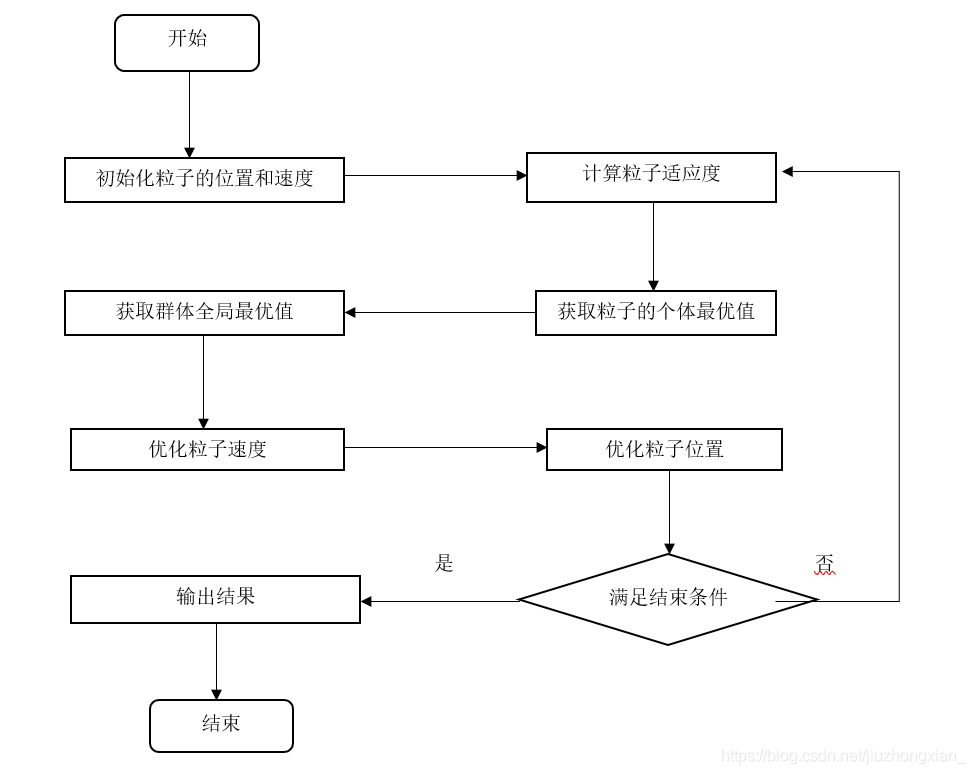
\includegraphics[width=0.9\textwidth]{figures/pso-flow.png}
    \caption{PSO算法流程图}
    \label{fig:pso_flow}
\end{figure}
\newpage
\section{总结}
粒子群算法的通用性较好,适合处理多种类型的目标函数约束问题,并且容易与传统的优化方法相结合,从而改进自身的局限性,更高效的解决问题,该算法具有随机性,故每次所求结果可能不同。



